\input{template}
\title{\bfseries 基于 SVD 的图像压缩与重构算法}
\author{韦晏洲 \quad PB24000379}

\begin{document}
	\maketitle
	\begin{abstract}
		本实验深入探讨了奇异值分解（SVD）在彩色图像压缩与重构中的应用。通过将 RGB 图像分解为独立颜色通道并采用 Jacobi 旋转法实现 SVD，利用矩阵的低秩近似）在大幅降低数据存储量的同时保留图像关键特征。实验选取多种不同复杂度的图像进行处理，并定量分析了截断秩 $k$ 对压缩率 $\rho$、峰值信噪比（PSNR）及结构相似性（SSIM）的影响。研究结果表明，自然图像的奇异值 $\sigma$ 呈现显著的“长尾衰减”特性，在 $k=50$ 左右即可实现高保真度的视觉重构；对比实验揭示，随机噪声图像（雪花图）因其高熵属性导致奇异值分布均匀、能量分散，难以通过低秩近似有效压缩。本实验通过构建基于 Streamlit 的交互式平台，在实时图像处理中直观展示了算法。
	\end{abstract}
	\clearpage

	\section{问题分析}
	
	本实验旨在探索奇异值分解（SVD）在彩色图像压缩中的应用。通过将图像抽象为数学上的矩阵，利用 SVD 提取其主要特征分量，从而在保证视觉质量的前提下实现数据压缩。
	
	\subsection{图像的矩阵表示与彩色图像处理}
	在计算机视觉中，数字图像本质上是一个离散的像素网格。
	\begin{itemize}
		\item \textbf{矩阵表示}：对于一副分辨率为 $M \times N$ 的数字图像，其每个像素点的亮度信息可以用一个数值表示（通常为 $0-255$或$0-65535$）。因此，单通道图像可以对应一个 $M \times N$ 的实数矩阵 $A$。
		
		\item \textbf{彩色图像处理}：本任务重点处理彩色图像。彩色图像通常基于 RGB 色彩空间，可以视为一个 $M \times N \times 3$ 的三阶张量。在实际操作中，我们将图像分解为红色（R）、绿色（G）、蓝色（B）三个独立的颜色通道，每个通道分别作为一个独立的 $M \times N$ 矩阵进行 SVD 分解和压缩处理，最后再将处理后的三个通道合并还原。
	\end{itemize}
	
	\subsection{SVD 分解的物理意义：低秩近似}
	奇异值分解不仅仅是一个数学公式 $A = U \Sigma V^T$，它更揭示了矩阵中隐含的结构信息。
	\begin{itemize}
		\item \textbf{能量分布}：矩阵 $A$ 可以表示为一系列秩为 1 的“小矩阵”之和：
		\begin{equation*}
			A = \sum_{i=1}^{r} \sigma_i u_i v_i^T
		\end{equation*}
		其中奇异值 $\sigma_i$ 衡量了这些“小矩阵”对于原矩阵 $A$ 的权重（即信息量）。在自然图像中，奇异值的分布通常呈现极强的“长尾效应”，即少数较大的奇异值集中了图像绝大部分的能量（轮廓、主要色彩），而大量的微小奇异值则对应噪声或极其微小的细节。
		\item \textbf{压缩原理}：通过保留前 $k$ 个最大的奇异值（$k \ll r$），我们可以构造原矩阵的最佳低秩近似 $A_k$。这在物理意义上相当于舍弃了图像中不重要的微弱信息，从而显著降低了存储空间的需求。
	\end{itemize}
	
	\subsection{图像质量评价指标}
	为了客观衡量压缩算法的效果，我们引入以下核心指标:
		
	\subsubsection{压缩率 (Compression Rate)}
	为了更直观地衡量压缩后数据量相对于原始数据的占比，我们引入压缩率 $\rho$。与压缩比不同，压缩率 $\rho \le 1$ 越小，说明压缩效果越显著，节省的存储空间越多。
	
	对于一幅分辨率为 $m \times n$、通道数为 $c$（RGB 图像 $c=3$）的原始图像，其总数据量为：
	\begin{equation*}
		S_{origin} = m \times n \times c
	\end{equation*}
	
	在 SVD 压缩方案中，若我们保留前 $k$ 个奇异值进行低秩近似，则每个通道需要存储 $U_k$ ($m \times k$)、$\Sigma_k$ ($k$ 个对角元) 和 $V_k^T$ ($k \times n$)。因此，压缩后的总存储数据量为：
	\begin{equation*}
		S_{compressed} = k(m + n + 1) \times c
	\end{equation*}
	
	综上所述，SVD 图像压缩的压缩率 $\rho$ 计算公式为：
	\begin{equation*}
		\rho = \frac{S_{compressed}}{S_{origin}} = \frac{k \times (m + n + 1) \times c}{m \times n \times c} = \frac{k(m + n + 1)}{mn}
	\end{equation*}
	
	\subsubsection{峰值信噪比 (PSNR)}
	PSNR 是基于均方误差（MSE）定义的客观标准，单位为分贝（dB）。对于彩色图像，其计算公式为：
	\begin{equation*}
		MSE = \frac{1}{\text{\#channel} \ M N} \sum_{c \in \text{channel}} \sum_{i=1}^{M} \sum_{j=1}^{N} [I_c(i,j) - \hat{I}_c(i,j)]^2
	\end{equation*}
	\begin{equation*}
		PSNR = 10 \cdot \log_{10} \left( \frac{\text{\#color}^2}{MSE} \right)
	\end{equation*}
	其中 \#color 为图像像素的最大值（一般为 255 或 65535）， channel 一般为 \{R,G,B\}。PSNR 值越高，表示图像失真越小。
	
	\subsubsection{结构相似性指数 (SSIM)}
	与 PSNR 仅考虑像素点误差不同，SSIM 更符合人类视觉系统的感知特性。它假设人类视觉能高度提取场景中的结构信息，因此采用一个大小为 $N \times N$ 的滑动窗口（如 $11 \times 11$），计算局部区域的指标：
	
	\begin{enumerate}
		\item \textbf{亮度比较 (Luminance)}：用均值 $\mu$ 表示。对于窗口内的像素集 $x$，其均值定义为：
		\begin{equation*}
			\mu_x = \frac{1}{N^2} \sum_{i=1}^{N^2} x_i
		\end{equation*}
		
		\item \textbf{对比度比较 (Contrast)}：用标准差 $\sigma$ 表示。它反映了图像像素值的幅度变化：
		\begin{equation*}
			\sigma_x = \sqrt{\frac{1}{N^2-1} \sum_{i=1}^{N^2} (x_i - \mu_x)^2}
		\end{equation*}
		
		\item \textbf{结构比较 (Structure)}：用协方差 $\sigma_{xy}$ 表示。它反映了两个信号结构上的相关性：
		\begin{equation*}
			\sigma_{xy} = \frac{1}{N^2-1} \sum_{i=1}^{N^2} (x_i - \mu_x)(y_i - \mu_y)
		\end{equation*}
	\end{enumerate}
	
	为了防止分母为 0 导致数值不稳定，引入常数 $C_1, C_2$：
	\begin{itemize}
		\item $C_1 = (k_1 L)^2$，$C_2 = (k_2 L)^2$。
		\item 其中 $L$ 是像素值的动态范围（对于 8-bit 图像，$L=255$）。
		\item $k_1, k_2$ 是默认常数，通常取 $k_1=0.01, k_2=0.03$。
	\end{itemize}
	
	最终的 SSIM 计算公式简化为：
	\begin{equation*}
		SSIM(x,y) = \frac{(2\mu_x\mu_y + C_1)(2\sigma_{xy} + C_2)}{(\mu_x^2 + \mu_y^2 + C_1)(\sigma_x^2 + \sigma_y^2 + C_2)}
	\end{equation*}
	
	在实际应用中，全图的 SSIM 分数通常是所有局部窗口 SSIM 值的平均值（Mean SSIM, MSSIM）。其值范围为 $[0, 1]$，越接近 1 说明两张图在结构和视觉感受上越一致。

	\section{算法与实现}
	
	\subsection{对称实矩阵特征系统求解}
	
	在实现SVD分解算法之前，我们需要完成对称实矩阵 $C \in \mathbb{R}^{n\times n}$ 的所有特征值与特征向量求解。我们采用数值线性代数中的\textit{Jacobi旋转法}。	
	在实际算法中取 $\eps = 10^{-6} \times\text{\#color}^2, \  T = 5N^2$ 处理 $N \times N$ 的矩阵。很遗憾，此方法处理 $N = 640$ 的图像需要3分钟以上时间。
	
	\begin{algorithm}[H]
		\caption{Jacobi 旋转法求解对称矩阵特征值与特征向量}
		\label{alg:jacobi}
		\begin{algorithmic}[1]
			\Require 对称矩阵 $C \in \mathbb{R}^{n \times n}$，收敛阈值 $\varepsilon$，最大迭代次数 $T$
			\Ensure 特征值 $\lambda_1, \dots, \lambda_n$ 及其对应的特征向量矩阵 $V$
			
			\State 初始化特征向量矩阵 $V = I$ （$n \times n$ 单位矩阵）
			\For{$iter = 1$ \textbf{to} $T$}
			\State \textbf{Step 1: 寻找旋转位置}
			\State 寻找非对角线绝对值最大的元素 $C_{pq}$，使得 $|C_{pq}| = \max_{i \neq j} |C_{ij}|$
			\If{$|C_{pq}| < \varepsilon$} 
			\State \textbf{break} \Comment{非对角线元素已足够小，算法收敛}
			\EndIf
			\State
			\State \textbf{Step 2: 计算旋转参数}
			\State $\tau = \frac{C_{qq} - C_{pp}}{2C_{pq}}$
			\State $t = \frac{\text{sgn}(\tau)}{|\tau| + \sqrt{1 + \tau^2}}$ \Comment{计算 $\tan \theta$}
			\State $c = \frac{1}{\sqrt{1 + t^2}}$, \quad $s = c \cdot t$ \Comment{计算 $\cos \theta$ 和 $\sin \theta$}
			\State
			\State \textbf{Step 3: 更新矩阵 $C$ （执行 $C \leftarrow P^T C P$）}
			\State 保存旧值：$C_{pp}^{old} = C_{pp}$, \quad $C_{qq}^{old} = C_{qq}$
			\State $C_{pp} = c^2 C_{pp}^{old} + s^2 C_{qq}^{old} - 2sc C_{pq}$
			\State $C_{qq} = s^2 C_{pp}^{old} + c^2 C_{qq}^{old} + 2sc C_{pq}$
			\State $C_{pq} = C_{qp} = 0$
			\For{$k = 1$ \textbf{to} $n$, 且 $k \neq p, q$}
			\State $C_{pk}^{new} = c C_{pk} - s C_{qk}$
			\State $C_{qk}^{new} = s C_{pk} + c C_{qk}$
			\State $C_{pk} = C_{kp} = C_{pk}^{new}$
			\State $C_{qk} = C_{kq} = C_{qk}^{new}$
			\EndFor
			\State
			\State \textbf{Step 4: 更新特征向量矩阵 $V$ （执行 $V \leftarrow V P$）}
			\For{$k = 1$ \textbf{to} $n$}
			\State $V_{kp}^{new} = c V_{kp} - s V_{kq}$
			\State $V_{kq}^{new} = s V_{kp} + c V_{kq}$
			\State $V_{kp} = V_{kp}^{new}, \quad V_{kq} = V_{kq}^{new}$
			\EndFor
			\EndFor
			\State 提取 $C$ 的对角线元素作为特征值 $\lambda_i = C_{ii}$
			\State 将 $\lambda_i$ 按降序排列，并同步调整 $V$ 的列顺序
			\State \Return $[\lambda_1 \cdots \lambda_n], V$
		\end{algorithmic}
	\end{algorithm}
	
	标准的Jacobi迭代法之所以很慢，是因为每进行一次旋转都要从矩阵的 $\frac{N^2 - N}{2}$ 个上三角元素中寻找最大值，而每一次旋转的计算开销仅为 $\mathcal{O}(N)$，当$N$很大时前者的开销已经超过了后者。对此我们引入\textit{动态阈值方法}，这是数值线性代数的另一标准优化方法。我们取 $\eps = 10^{-6} \times \text{\#color}$, $T=20$。此方法处理 $ N = 640$ 的图像只需要1分钟时间，但是仍然较长。
	
	\begin{algorithm}[H]
		\caption{动态阈值Jacobi旋转法}
		\label{alg:optimized_jacobi}
		\begin{algorithmic}[1]
			\Require 对称矩阵 $C \in \mathbb{R}^{n \times n}$，最终收敛阈值 $\varepsilon$，最大圈数 $T$
			\Ensure 降序排列的特征值 $\lambda$ 及其特征向量矩阵 $V$
			
			\State 初始化 $V = I_n$
			\For{$sweep = 1$ \textbf{to} $T$}
			\State \textbf{Step 1: 计算当前圈的动态阈值}
			\State $max\_off\_val = \max_{i < j} |C_{ij}|$
			\If{$max\_off\_val < \varepsilon$} 
			\State \textbf{break} \Comment{全局已达到收敛精度}
			\EndIf
			\State $thresh = \max(\varepsilon, max\_off\_val \times 0.2)$ \Comment{跳过非核心旋转}
			\State
			\State \textbf{Step 2: 循环扫描所有非对角元素}
			\For{$p = 1$ \textbf{to} $n - 1$}
			\For{$q = p + 1$ \textbf{to} $n$}
			\If{$|C_{pq}| \le thresh$} \textbf{continue} \Comment{核心优化点}
			\EndIf
			\State \textbf{Step 3: 计算旋转矩阵参数, Step 4: 原地更新，同\ref{alg:jacobi}}
			\EndFor
			\EndFor
			\EndFor
			\State \Return $\text{sort}(\text{diag}(C)), V$ （按特征值降序对齐）
		\end{algorithmic}
	\end{algorithm}

	为了进一步压榨计算性能，我们采用了基于 \textbf{Numba} 的即时编译技术对算法进行底层重构。由于本人没有学过计算机系统相关课程，故对优化原理并不了解。不过在使用该库后，处理 $N \times N$ 图像 $(N = 640)$ 的时间降至 $5s$，优化效果非常明显。
	
	\subsection{SVD分解算法}
	
	考虑经典 SVD 分解算法

	\begin{algorithm}[H]
		\caption{SVD 分解算法}
		\label{alg:svd}
		\begin{algorithmic}[1]
			\State \textbf{Input:} 矩阵 $A \in \mathbb{R}^{m \times n}$
			\State \textbf{Output:} $U, \Sigma, V^T$
			\State
			\State \textbf{Step 1: 计算对称矩阵}
			\State 计算 $C = A^T A$ （结果为 $n \times n$ 矩阵）。
			\State
			\State \textbf{Step 2: 求解特征值与特征向量 ($V$)}
			\State 使用\ref{alg:jacobi}中的 Jacobi 旋转法求 $C$ 的特征值 $\lambda_i$ 和特征向量 $v_i$。
			\State 将特征值按降序排列：$\lambda_1 \ge \lambda_2 \ge \dots \ge \lambda_n$。
			\State 对应的特征向量构成矩阵 $V = [v_1, v_2, \dots, v_n]$。
			\State
			\State \textbf{Step 3: 构造奇异值矩阵 ($\Sigma$)}
			\State 计算奇异值 $\sigma_i = \sqrt{\lambda_i}$。
			\State 构造 $m \times n$ 的对角矩阵 $\Sigma$，其对角元 $\Sigma_{ii} = \sigma_i$。
			\State
			\State \textbf{Step 4: 求解左奇异矩阵 ($U$)}
			\State 对于每个非零奇异值 $\sigma_i$，计算 $u_i = \frac{1}{\sigma_i} A v_i$。
			\State 若 $m > n$，需利用施密特正交化补全 $U$ 的其余列向量，使其成为正交矩阵。
			\State
			\State \textbf{Return:} $U, \Sigma, V^T$
		\end{algorithmic}
	\end{algorithm}
	
	我们使用一张尺寸为$1170 \times 2601$的图片进行测试，运行时长大约为150s, 这是由于 $C = A^T A \in \mathbb{R}^{2601 \times 2601}$ 包含了大量零特征值，且后续施密特正交化也浪费了大量算力。对此，我们对输入的 $A$ 的形状进行判断，再决定选用 $A^T A$ 还是 $AA^T$ 做特征系统求解。在此优化下，我们无需做施密特正交化，求解该图片仅用时12s，实现了极大的优化。
	
	\begin{algorithm}[H]
		\caption{基于矩阵形状优化的 SVD 分解算法}
		\label{alg:svd_optimized}
		\begin{algorithmic}[1]
			\Require 矩阵 $A \in \mathbb{R}^{m \times n}$，目标秩 $k$
			\Ensure 左奇异矩阵 $U$，奇异值向量 $\sigma$，右奇异矩阵 $V^T$
			\State
			\If{$m \ge n$} \Comment{高瘦型矩阵，优先求解 $V$}
			\State \textbf{Step 1:} 计算协方差矩阵 $C = A^T A \in \mathbb{R}^{n \times n}$
			\State \textbf{Step 2:} 调用算法\ref{alg:jacobi}求解 $C$ 的特征值 $\lambda_i$ 与特征向量 $v_i$
			\State \textbf{Step 3:} 计算奇异值 $\sigma_i = \sqrt{\max(\lambda_i, 0)}$，排列为对角矩阵$\Sigma$
			\State \textbf{Step 4:} 构造 $V = [v_1, \dots, v_n]$
			\State \textbf{Step 5:} 通过公式 $u_i = \frac{1}{\sigma_i} A v_i$ 向量化求解 $U = A V \Sigma^{-1}$
			\Else \Comment{矮胖型矩阵，优先求解 $U$}
			\State \textbf{Step 1:} 计算协方差矩阵 $C = A A^T \in \mathbb{R}^{m \times m}$
			\State \textbf{Step 2:} 调用算法\ref{alg:jacobi}求解 $C$ 的特征值 $\lambda_i$ 与特征向量 $u_i$
			\State \textbf{Step 3:} 计算奇异值 $\sigma_i = \sqrt{\max(\lambda_i, 0)}$，排列为对角矩阵$\Sigma$
			\State \textbf{Step 4:} 构造 $U = [u_1, \dots, u_m]$
			\State \textbf{Step 5:} 通过公式 $v_i = \frac{1}{\sigma_i} A^T u_i$ 向量化求解 $V = A^T U \Sigma^{-1}$
			\EndIf
			\State
			\State \Return $U, \Sigma, V^T$
		\end{algorithmic}
	\end{algorithm}
	
	\begin{rmk}
		在图像压缩的实际工程实现中，我们并不需要算法 \ref{alg:svd}, \ref{alg:svd_optimized} 产生的全量分解结果。为了获得秩-$k$ 近似矩阵 $[U_k, \Sigma_k, V_k^T]$，我们只需对上述算法进行裁剪即可。
		
	\end{rmk}
	
	在本实验中，我们希望看到 $k$ 从 1 到 $\min\{m,n\}$ 之间的连续变化，故实验进行了完整的SVD分解。
	
	\subsection{图像压缩算法}
	
	\begin{algorithm}[H]
		\caption{基于 SVD 的图像压缩与重构算法}
		\label{alg:svd_compression}
		\begin{algorithmic}[1]
			\Require 原始图像矩阵 $I \in \mathbb{R}^{m \times n \times c}$. 对RGB图像 $c = 3$，压缩秩 $k$
			\Ensure 重构后的图像 $I_{rec}$，压缩比 $\eta$，峰值信噪比 $PSNR$
			\State \textbf{Step 1: 图像预处理}
			\State 将图像分解为三个颜色通道矩阵：$I_R, I_G, I_B \in \mathbb{R}^{m \times n}$
			\State 设每个通道颜色数量为 \#color
			\State \textbf{Step 2: 对各通道进行低秩 SVD 近似}
			\For{每个通道矩阵 $A \in \{I_{R}, I_{G}, I_{B}\}$}
			\State 1. 截断：$[U_k, \Sigma_k, V_k^T] = \text{Truncate}[U, \Sigma, V]$，在求SVD分解的时候进行截断
			\State 2. 计算重构矩阵：$A' = U_k \cdot \text{diag}(\Sigma_k) \cdot V_k^T$
			\EndFor
			\State
			\State \textbf{Step 3: 图像合成与后处理}
			\State 合并各通道 $A'$ 得到重构矩阵 $I'_{raw}$
			\State $I_{rec} = \text{clip}(I'_{raw}, 0, \text{\#colour})$ \Comment{避免浮点数计算误差导致溢出}
			\State
			\State \textbf{Step 4: 性能评价指标计算}
			\State 1. 计算压缩率 (Compression Rate)：
			\State \quad $\rho = \frac{k \times (m + n + 1)}{m \times n}$
			\State 2. 计算均方误差 (MSE)：
			\State \quad $MSE = \frac{1}{3mn} \sum_{c \in \{R,G,B\}} \sum_{i=1}^{m} \sum_{j=1}^{n} (I_{i,j,c} - I_{rec,i,j,c})^2$
			\State 3. 计算峰值信噪比 (PSNR)：
			\State \quad $PSNR = 10 \cdot \log_{10}\left(\frac{\text{\#color}^2}{MSE}\right)$
			\State 4. 计算平均结构相似性 (MSSIM)：
			\For{每个通道 $c \in \{R, G, B\}$}
			\State (1) 将通道图像划分为 $M$ 个大小为 $N \times N$ 的局部窗口（如 $11 \times 11$）
			\State (2) 计算每个窗口 $j$ 的局部相似度：
			\State \quad $SSIM_j = \frac{(2\mu_{I,j}\mu_{rec,j} + C_1)(2\sigma_{I,rec,j} + C_2)}{(\mu_{I,j}^2 + \mu_{rec,j}^2 + C_1)(\sigma_{I,j}^2 + \sigma_{rec,j}^2 + C_2)}$
			\State (3) 该通道的平均相似度：$MSSIM_c = \frac{1}{M} \sum_{j=1}^M SSIM_j$
			\EndFor
			\State \quad 最终指标：$SSIM = \frac{1}{3} (MSSIM_R + MSSIM_G + MSSIM_B)$
			\State
			\State \Return $I_{rec}, \rho, PSNR, SSIM$
		\end{algorithmic}
	\end{algorithm}
	
	\subsection{界面设计}
	
	本实验通过构建基于 Streamlit 的交互式平台，直观展示了算法在图像处理的应用。在本地运行 Streamlit 时，需要在点击运行后在窗口输入 \texttt{python -m streamlit run app.py}，在浏览器中打开交互页面。
	
	\section{结果}
	
	\subsection{压缩结果}
	
	可以看出随着截断秩的提升，压缩率和指标PSNR, SSIM都稳步提升，图像复原度和清晰度也逐步提高。
	
	\begin{table}[htbp]
		\centering
		\caption{不同截断秩 $k$ 下的图像1压缩性能评价指标}
		\label{tab:svd_results}
		\begin{tabular}{@{}ccccc@{}}
			\toprule
			截断秩 $k$ & 压缩率 $\rho$ & PSNR (dB) & SSIM & 备注 \\ \toprule
			1   & 0.31\%   & 13.70  & 0.6029 & - \\
			5   & 1.56\%   & 20.09  & 0.6085 & 仅有轮廓 \\
			10  & 3.13\%   & 22.90  & 0.6255 & - \\
			20  & 6.25\%   & 25.99  & 0.6485 & 质量显著提升 \\
			50  & 15.64\%  & 31.46  & 0.7250 & 视觉无明显差异 \\
			100 & 31.27\%  & 36.41  & 0.7897 & 几乎看不出噪点 \\
			200 & 62.55\%  & 40.40  & 0.8242 & - \\
			640 & 200.16\% & 265.43 & 1.0000 & 完全重构 \\ \bottomrule
		\end{tabular}
	\end{table}
	
	对于电视机雪花图片图像（图像3）和高斯噪声图像（图像4），$k = 50$ 时 SSIM 只有0.6542和0.4015，低于正常图像（图像1），这是因为对于噪声高的图片，奇异值衰减更慢，也因此低秩截断效果更差。
	
	\begin{figure}[htbp]
		\centering
		% 第一行
		\begin{subfigure}[b]{0.3\textwidth}
			\centering
			
\includegraphics[width=\textwidth]{0.jpg}
			\caption{Original}
		\end{subfigure}
		\hfill
		\begin{subfigure}[b]{0.3\textwidth}
			\centering
			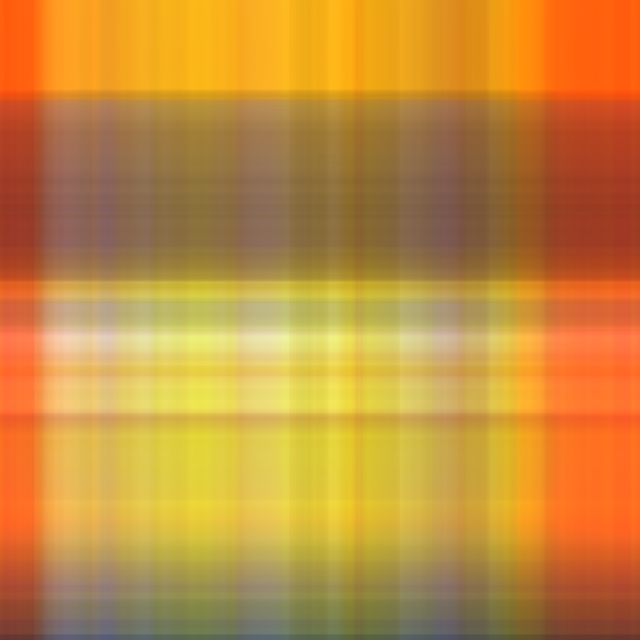
\includegraphics[width=\textwidth]{0-k1.png}
			\caption{$k=1$}
		\end{subfigure}
		\hfill
		\begin{subfigure}[b]{0.3\textwidth}
			\centering
			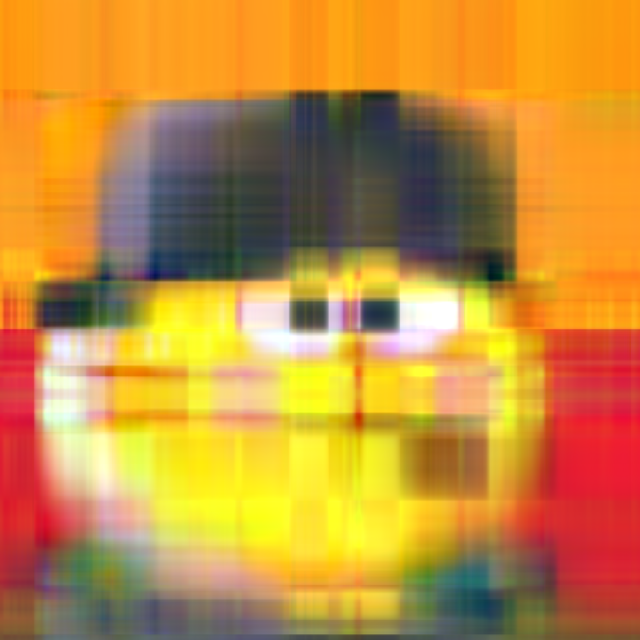
\includegraphics[width=\textwidth]{0-k5.png}
			\caption{$k=5$}
		\end{subfigure}
		
		\vspace{10pt}
		
		% 第二行
		\begin{subfigure}[b]{0.3\textwidth}
			\centering
			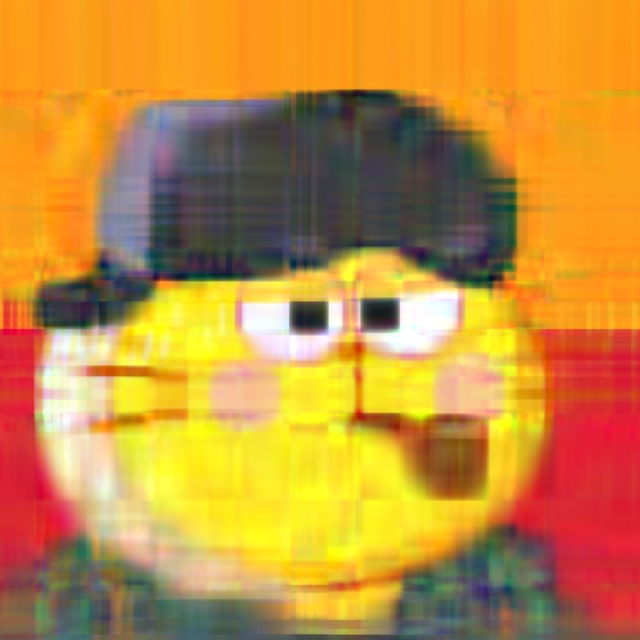
\includegraphics[width=\textwidth]{0-k10.png}
			\caption{$k=10$}
		\end{subfigure}
		\hfill
		\begin{subfigure}[b]{0.3\textwidth}
			\centering
			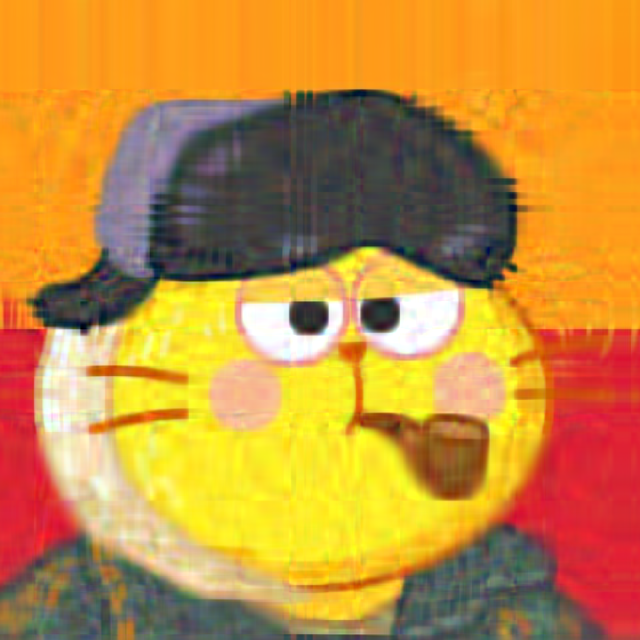
\includegraphics[width=\textwidth]{0-k20.png}
			\caption{$k=20$}
		\end{subfigure}
		\hfill
		\begin{subfigure}[b]{0.3\textwidth}
			\centering
			
\includegraphics[width=\textwidth]{0-k50.png}
			\caption{$k=50$}
		\end{subfigure}
		
		\vspace{10pt}
		
		% 第三行
		\begin{subfigure}[b]{0.3\textwidth}
			\centering
			
\includegraphics[width=\textwidth]{0-k100.png}
			\caption{$k=100$}
		\end{subfigure}
		\hfill
		\begin{subfigure}[b]{0.3\textwidth}
			\centering
			
\includegraphics[width=\textwidth]{0-k200.png}
			\caption{$k=200$}
		\end{subfigure}
		\hfill
		\begin{subfigure}[b]{0.3\textwidth}
			\centering
			
\includegraphics[width=\textwidth]{0-k640.png}
			\caption{$k=640$ (Full)}
		\end{subfigure}
		
		\caption{不同截断秩下图像压缩效果对比}
		\label{fig:svd_comparison}
	\end{figure}
	
		\begin{figure}[htbp]
		\centering
		% 左侧：原图
		\begin{subfigure}[b]{0.48\textwidth}
			\centering
			% 既然之前报错，这里稳妥起见依然加上双花括号，预防玄学报错
			\includegraphics[width=\textwidth]{{0.jpg}} 
			\caption{图像1 ($640 \times 640$)}
		\end{subfigure}
		\hfill % 在两图之间填充空白，强制它们左右对齐
		% 右侧：奇异值衰减图
		\begin{subfigure}[b]{0.48\textwidth}
			\centering
			\includegraphics[width=\textwidth]{{0-k50.png}}
			\caption{$k = 50$}
		\end{subfigure}
		
		\caption{图像1 ($640 \times 640$)分解效果}
		\end{figure}
		
	\begin{figure}[htbp]
		\centering
		% 左侧：原图
		\begin{subfigure}[b]{0.36\textwidth}
			\centering
			% 既然之前报错，这里稳妥起见依然加上双花括号，预防玄学报错
			\includegraphics[width=\textwidth]{{9.jpg}} 
			\caption{图像2 ($1073 \times 1822$)}
		\end{subfigure}
		\hfill % 在两图之间填充空白，强制它们左右对齐
		% 右侧：奇异值衰减图
		\begin{subfigure}[b]{0.36\textwidth}
			\centering
			\includegraphics[width=\textwidth]{{9-k50.png}}
			\caption{$k = 50$}
		\end{subfigure}
		\caption{图像2 ($1073 \times 1822$)分解效果}
	\end{figure}
	
	\begin{figure}[htbp]
		\centering
		% 左侧：原图
		\begin{subfigure}[b]{0.48\textwidth}
			\centering
			% 既然之前报错，这里稳妥起见依然加上双花括号，预防玄学报错
			\includegraphics[width=\textwidth]{{R.jpg}} 
			\caption{图像3 ($1920 \times 1080$)}
		\end{subfigure}
		\hfill % 在两图之间填充空白，强制它们左右对齐
		% 右侧：奇异值衰减图
		\begin{subfigure}[b]{0.48\textwidth}
			\centering
			\includegraphics[width=\textwidth]{{R-k50.png}}
			\caption{$k = 50$}
		\end{subfigure}
		\caption{图像3 ($1920 \times 1080$)分解效果}
	\end{figure}
	
	\begin{figure}[htbp]
		\centering
		% 左侧：原图
		\begin{subfigure}[b]{0.48\textwidth}
			\centering
			% 既然之前报错，这里稳妥起见依然加上双花括号，预防玄学报错
			\includegraphics[width=\textwidth]{{N.jpg}} 
			\caption{图像4 ($960 \times 1280$)}
		\end{subfigure}
		\hfill % 在两图之间填充空白，强制它们左右对齐
		% 右侧：奇异值衰减图
		\begin{subfigure}[b]{0.48\textwidth}
			\centering
			\includegraphics[width=\textwidth]{{N-k50.png}}
			\caption{$k = 50$}
		\end{subfigure}
		\caption{图像4 ($960 \times 1280$)分解效果}
	\end{figure}
	
	\subsection{奇异值分布}
	
	为了探究奇异值的分布，我们额外添加了绘制R通道奇异值分布的功能。为了避免矩阵奇异，我们为每个奇异值加上了$1e-16$ 的小量（虽然证明接下来的实验中这一操作并不需要）。
	
	可以发现，对于普通图片，像素之间具有极强的相关性，其能量高度集中在几个主成分上。而图像3, 4为电视机雪花图和高斯噪声图，其像素之间相关性较低，可以发现除了最大奇异值外，其余奇异值相对同尺寸的图像较低，且衰减平缓得多，这一点在图像4中尤为明显。
	
	\begin{figure}[htbp]
		\centering
		% 左侧：原图
		\begin{subfigure}[b]{0.32\textwidth}
			\centering
			% 既然之前报错，这里稳妥起见依然加上双花括号，预防玄学报错
			\includegraphics[width=\textwidth]{{0.jpg}} 
			\caption{Original Image}
			\label{fig:orig_0}
		\end{subfigure}
		\hfill % 在两图之间填充空白，强制它们左右对齐
		% 右侧：奇异值衰减图
		\begin{subfigure}[b]{0.64\textwidth}
			\centering
			\includegraphics[width=\textwidth]{{0SVDecay.png}}
			\caption{Singular Value Distribution}
			\label{fig:decay_0}
		\end{subfigure}
		
		% 主标题和标签
		\caption{图像 1 ($640 \times 640$) 及其奇异值特征分析对比}
		\label{fig:0orig_vs_decay}
	\end{figure}
	
	\begin{figure}[htbp]
		\centering
		% 左侧：原图
		\begin{subfigure}[b]{0.32\textwidth}
			\centering
			% 既然之前报错，这里稳妥起见依然加上双花括号，预防玄学报错
			\includegraphics[width=\textwidth]{{9.jpg}} 
			\caption{Original Image}
			\label{fig:orig_9}
		\end{subfigure}
		\hfill % 在两图之间填充空白，强制它们左右对齐
		% 右侧：奇异值衰减图
		\begin{subfigure}[b]{0.64\textwidth}
			\centering
			\includegraphics[width=\textwidth]{{9SVDecay.png}}
			\caption{Singular Value Distribution}
			\label{fig:decay_9}
		\end{subfigure}
		
		% 主标题和标签
		\caption{图像 2 ($1822\times 1073$)及其奇异值特征分析对比}
		\label{fig:9orig_vs_decay}
	\end{figure}

	\begin{figure}[htbp]
		\centering
		% 左侧：原图
		\begin{subfigure}[b]{0.32\textwidth}
			\centering
			% 既然之前报错，这里稳妥起见依然加上双花括号，预防玄学报错
			\includegraphics[width=\textwidth]{{R.jpg}} 
			\caption{Original Image}
			\label{fig:orig_R}
		\end{subfigure}
		\hfill % 在两图之间填充空白，强制它们左右对齐
		% 右侧：奇异值衰减图
		\begin{subfigure}[b]{0.64\textwidth}
			\centering
			\includegraphics[width=\textwidth]{{RSVDecay.png}}
			\caption{Singular Value Distribution}
			\label{fig:decay_R}
		\end{subfigure}
		
		% 主标题和标签
		\caption{图像 3 ($1920 \times 1080$) 及其奇异值特征分析对比}
		\label{fig:Rorig_vs_decay}
	\end{figure}
	
		\begin{figure}[htbp]
		\centering
		% 左侧：原图
		\begin{subfigure}[b]{0.32\textwidth}
			\centering
			% 既然之前报错，这里稳妥起见依然加上双花括号，预防玄学报错
			\includegraphics[width=\textwidth]{{N.jpg}} 
			\caption{Original Image}
			\label{fig:orig_N}
		\end{subfigure}
		\hfill % 在两图之间填充空白，强制它们左右对齐
		% 右侧：奇异值衰减图
		\begin{subfigure}[b]{0.64\textwidth}
			\centering
			\includegraphics[width=\textwidth]{{NSVDecay.png}}
			\caption{Singular Value Distribution}
			\label{fig:decay_N}
		\end{subfigure}
		
		% 主标题和标签
		\caption{图像 4 ($960 \times 1280$) 及其奇异值特征分析对比}
		\label{fig:Norig_vs_decay}
	\end{figure}

\end{document}


